%-what did we achieve?\\
% *managing scv units harvesting and building using Markov chains\\
% *system for buildings to train units using Markov chains

\begin{figure}[ht]
\centering
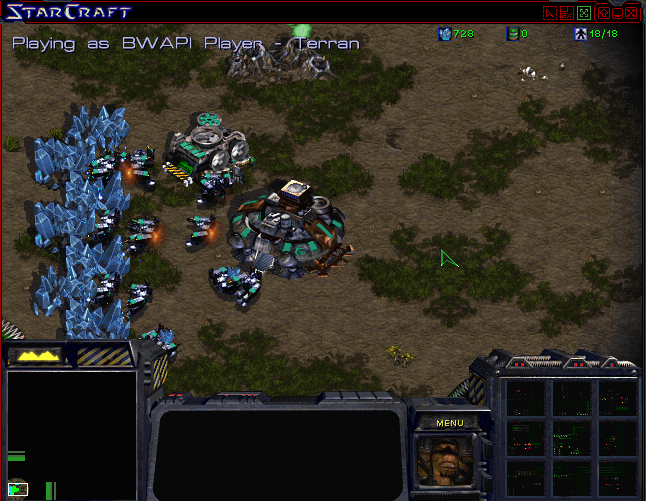
\includegraphics[scale=0.6, trim = 0cm 0cm 0cm 0.0cm]{images/Victory}
\label{fig:gameplay}
\caption{A screenshot of our agents gathering resources and some of the buildings they have constructed.}
\end{figure}


In the end we had a system for controlling SCV units and buildings using Markov chains which were influenced by the currently available unit slots and resources. Managing the splitting the SCV units between constructing buildings and harvesting and the point at which buildings created units were controlled by parameters the system could learn. The unit and base constructing and resource gathering aspects of the game could all be handled using Markov chains. Figure~\ref{fig:gameplay} shows an early stage of the game where SCVs are harvesting and have built a few buildings.

%-have we any way of evaluating our performance?\\
% *number of units and buildings completed after n-minutes?\\
% *needs to be somehow combined with a full strategy for proper evaluation (more in conclusion)..

 The problem we encountered was trying to decide on a way of evaluating the performance of our bot. The number and type of buildings and units on it's own is not a great performance metric. It would just result in the bot converging on optimum parameters to satisfy what is considered the best.

 The system could be paired with another agent to handle offensive capabilities but then the solution would choose optimum values for that bot and maybe even a specific enemy.

 Another method would be to compare the time at which we reach certain research levels and the unit output of our bot against the time that of other bots take to do the same.